\section{Desarrollo protocolo de control in-band}
\label{sec:bofussDEV}


En esta sección se va a explicar la implementación realizada del protocolo Iotorii en el \textit{software switch} de \gls{bofus}. Dado que el trabajo de implementación ha sido bastante extenso, dado que había que discernir que parte de la implementación del control in-band podía ser aprovechada, se ha decidido generar un documento anexo \cite{davidBOFUSS} aparte de la memoria, donde se explique a bajo nivel las modificaciones realizadas. Todo el código se puede encontrar indicado en la Sección \ref{sec:estadoArte_github}. \\
\\
En la Figura \ref{}, se puede apreciar la secuencia lógica que se ha llevado a cabo para la implementación del protocolo Iotorii en el software switch. En primer lugar, se han detectado todas las modificaciones realizadas anteriormente en la implementación del control in-band llevada a cabo por mi compañero Boby,


% fig
\begin{figure}[ht]
    \centering
    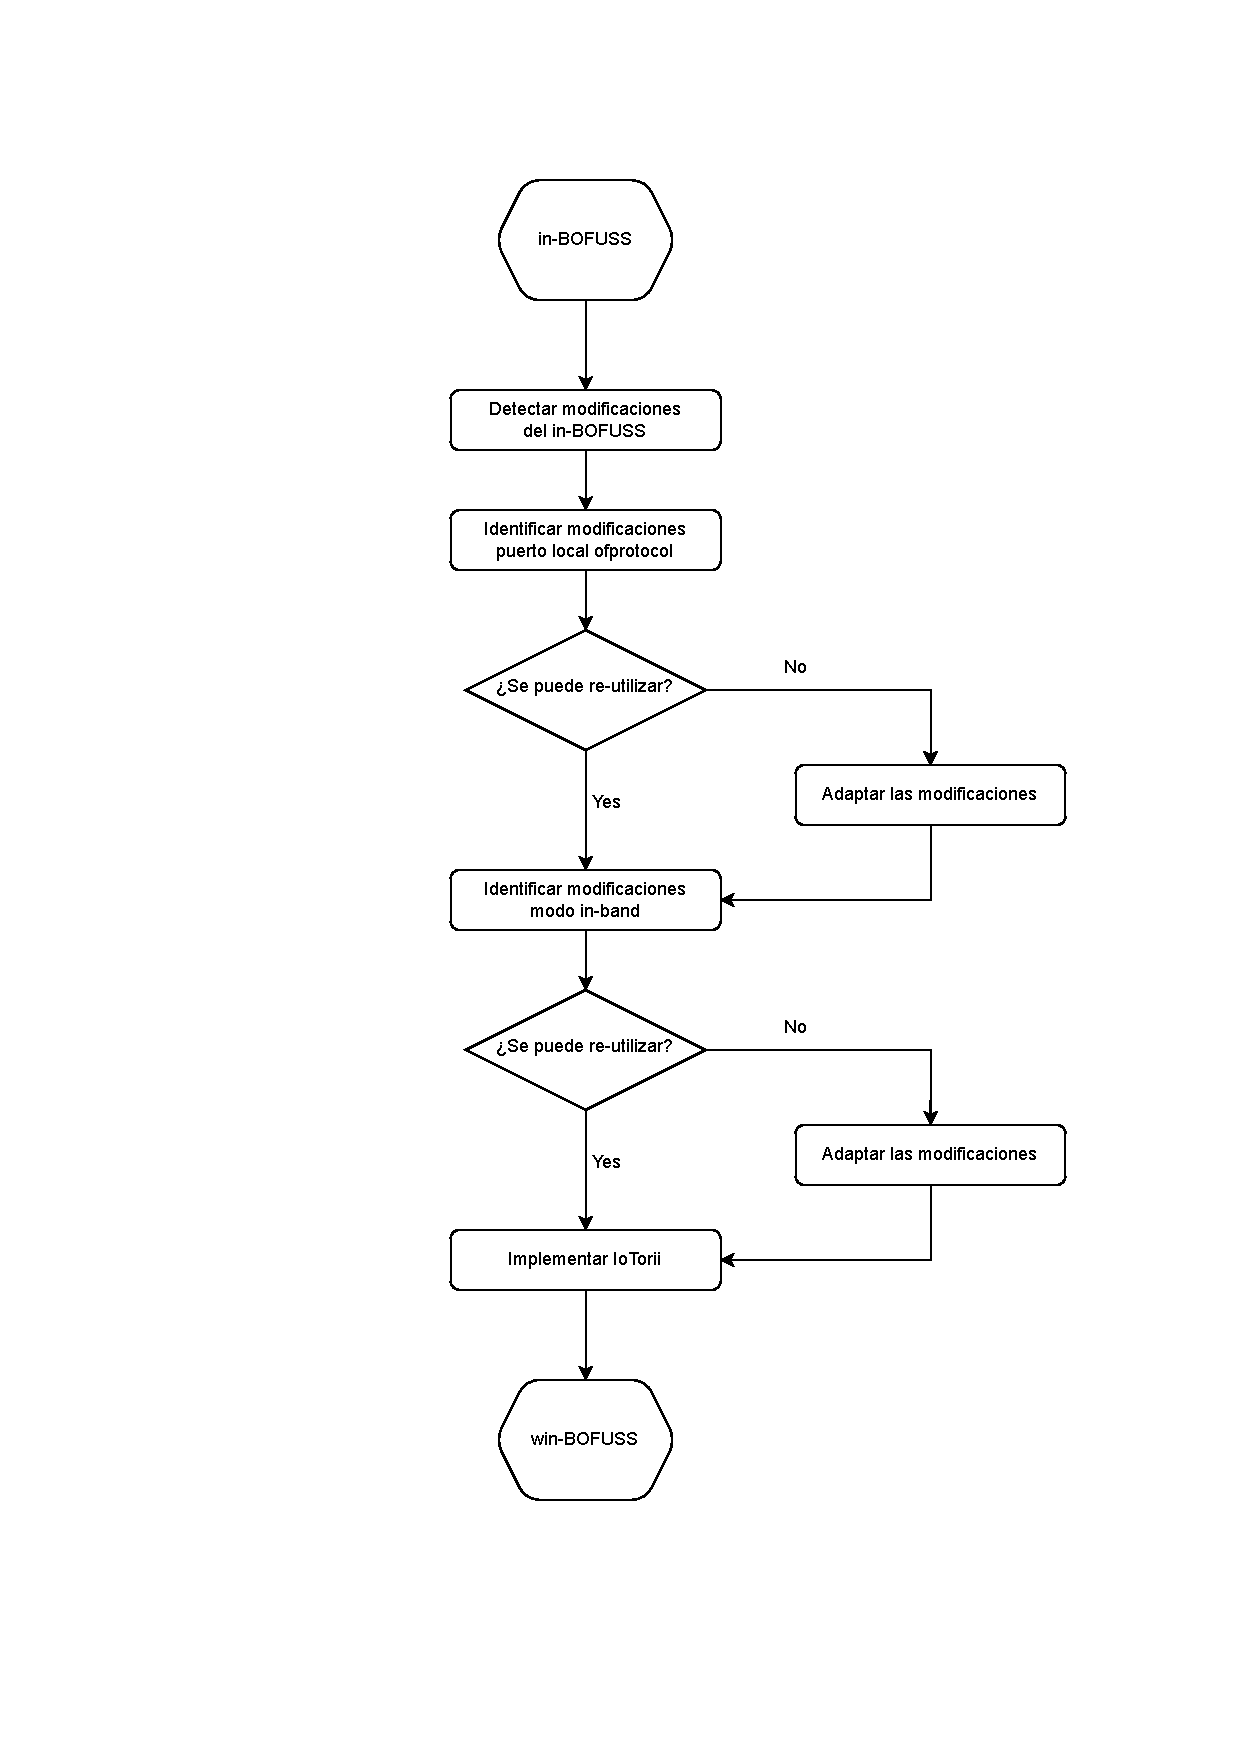
\includegraphics[width=\textwidth]{archivos/img/dev/WIN-BOFUSS.drawio.pdf}
    \caption{\textit{Rollback} a la nueva herramienta \texttt{dpctl}}
    \label{fig:WIN-BOFUSS}
\end{figure}


